%\VignetteIndexEntry{Randomization-based inference}
%\VignettePackage{mosaic}
%\VignetteKeywords{mosaic, resampling, bootstrapping, permutation}
%\VignetteEngine{knitr::knitr} 

\documentclass[11pt]{article}\usepackage[]{graphicx}\usepackage[]{color}
% maxwidth is the original width if it is less than linewidth
% otherwise use linewidth (to make sure the graphics do not exceed the margin)
\makeatletter
\def\maxwidth{ %
  \ifdim\Gin@nat@width>\linewidth
    \linewidth
  \else
    \Gin@nat@width
  \fi
}
\makeatother

\definecolor{fgcolor}{rgb}{0.345, 0.345, 0.345}
\newcommand{\hlnum}[1]{\textcolor[rgb]{0.686,0.059,0.569}{#1}}%
\newcommand{\hlstr}[1]{\textcolor[rgb]{0.192,0.494,0.8}{#1}}%
\newcommand{\hlcom}[1]{\textcolor[rgb]{0.678,0.584,0.686}{\textit{#1}}}%
\newcommand{\hlopt}[1]{\textcolor[rgb]{0,0,0}{#1}}%
\newcommand{\hlstd}[1]{\textcolor[rgb]{0.345,0.345,0.345}{#1}}%
\newcommand{\hlkwa}[1]{\textcolor[rgb]{0.161,0.373,0.58}{\textbf{#1}}}%
\newcommand{\hlkwb}[1]{\textcolor[rgb]{0.69,0.353,0.396}{#1}}%
\newcommand{\hlkwc}[1]{\textcolor[rgb]{0.333,0.667,0.333}{#1}}%
\newcommand{\hlkwd}[1]{\textcolor[rgb]{0.737,0.353,0.396}{\textbf{#1}}}%
\let\hlipl\hlkwb

\usepackage{framed}
\makeatletter
\newenvironment{kframe}{%
 \def\at@end@of@kframe{}%
 \ifinner\ifhmode%
  \def\at@end@of@kframe{\end{minipage}}%
  \begin{minipage}{\columnwidth}%
 \fi\fi%
 \def\FrameCommand##1{\hskip\@totalleftmargin \hskip-\fboxsep
 \colorbox{shadecolor}{##1}\hskip-\fboxsep
     % There is no \\@totalrightmargin, so:
     \hskip-\linewidth \hskip-\@totalleftmargin \hskip\columnwidth}%
 \MakeFramed {\advance\hsize-\width
   \@totalleftmargin\z@ \linewidth\hsize
   \@setminipage}}%
 {\par\unskip\endMakeFramed%
 \at@end@of@kframe}
\makeatother

\definecolor{shadecolor}{rgb}{.97, .97, .97}
\definecolor{messagecolor}{rgb}{0, 0, 0}
\definecolor{warningcolor}{rgb}{1, 0, 1}
\definecolor{errorcolor}{rgb}{1, 0, 0}
\newenvironment{knitrout}{}{} % an empty environment to be redefined in TeX

\usepackage{alltt}
\usepackage{mosaic}
\usepackage{graphicx}
\usepackage{amsmath}
\usepackage{amsfonts}
\usepackage{amssymb}
%\usepackage{epstopdf}
%\usepackage{color}
\usepackage{url}
\usepackage{hyperref} 
\usepackage[margin=1in]{geometry}
%\usepackage[parfill]{parskip}
\hypersetup{pdftitle={Resampling-based inference}, colorlinks=true, linkcolor=black, citecolor=black}
%\usepackage[bottom]{footmisc}
%\usepackage[round]{natbib}
\bibliographystyle{abbrvnat}

\frenchspacing{}

\title{Randomization-based inference using the {\tt mosaic} package}
\author{Daniel Kaplan\thanks{dtkaplan@gmail.com} \\ \footnotesize Macalester College \\
\footnotesize St. Paul, MN
\and Nicholas J. Horton\thanks{nhorton@amherst.edu} \\ \footnotesize Amherst College \\
\footnotesize Amherst, MA \and 
Randall Pruim\thanks{rpruim@calvin.edu}
\\ \footnotesize Calvin College \\
\footnotesize Grand Rapids, MI
}
\date{\today}
\IfFileExists{upquote.sty}{\usepackage{upquote}}{}
\begin{document}
%\SweaveOpts{concordance=TRUE}

\maketitle

\tableofcontents





\section{Introduction}

The \pkg{mosaic} package is intended to support teaching statistics and modeling (as well as calculus) in a way that embraces the possibilities offered by modern computational techniques.
Our goal is to make effective computation accessible to university-level students at an introductory level.  With the broad availability of inexpensive, fast computing and powerful, free software such as \R, the rate-limiting factor in accessibility is intellectual: providing a notation in which ideas can be expressed and understood clearly.  

This document describes how to use the \pkg{mosaic} package to carry out randomization-based statistical inference.  The \pkg{mosaic} package supports an approach that is intended to be easy for students to learn and to generalize.  To this end, we adopt the following tenets:
\begin{itemize}
\item Students should be able to carry out useful statistics with only a very few lines of commands.
\item Basic commands should relate to statistical operations rather than programming operations.  We seek to avoid programming overhead such as loops, counters, and accumulators.
\item Black boxes should perform a conceptually straightforward operations.  Their output should be verifiable.
\item Statements should demonstrate the logical structure of statistics, rather than merely naming high-level procedures.
\item There should be a simple path to generalizing from simple descriptions --- means, counts, proportions --- to more complicated ones such as generalized linear models.
\end{itemize}

The \pkg{mosaic} operations allow students to implement each of the
operations in what George Cobb calls the ``3 Rs'' of statistical
inference: Randomization, Replication, and Rejection (Cobb, 2007). 
By putting the 3 Rs together in various ways, students learn to
generalize and internalize the logic of inference, rather than just
to blindly follow formulaic methods.

Terry Speed (2011) notes the changing role of simulation in statistics.  :
\begin{quote}
[Simulation used to be] something that people did when they can't do the math. $\ldots$ It now seems
that we are heading into an era when all statistical analysis can be done by
simulation.
\end{quote}

Arguably, the most important operation in statistics is sampling:
ideally, selecting a random subset from a population.  Regrettably,
sampling takes work and time, so instructors tend to de-emphasize the
actual practice of sampling in favor of theoretical descriptions.
What's more, the algebraic notation in which much of conventional
textbook statistics is written does not offer an obvious notation for sampling.

With the computer, however, these efficiency and notation obstacles
can be overcome.  Sampling can be placed in its rightfully central
place among the statistical concepts in our courses.

Randomization-based inference using permutation testing and bootstrapping are an
increasingly important set of techniques for introductory statistics and beyond.
To help educators usefully compare different software approaches, 
Robin Lock and colleagues posed a series of problems at USCOTS 2011 
(United States Conference on Teaching Statistics), 
as described at \url{http://www.causeweb.org/uscots/breakout/breakout3_6.php}, 
relating to bootstrapping and permutation tests. 
Bootstrapping and permutation testing are powerful and elegant approaches to
estimation and testing that can be implemented even in many
situations where asymptotic results are difficult to find or otherwise
unsatisfactory (Efron and Tibshirani, 1993; Hesterberg et al 2005).
Bootstrapping involves sampling \emph{with} replacement from a population,
repeatedly calculating a sample statistic of interest to empirically construct
the sampling distribution. Permutation testing for a two group comparison is
done by \emph{permuting} the labels for the grouping variable, then calculating
the sample statistic (e.g. difference between two groups using these new
labels) to empirically construct the null distribution. 

We will illustrate the use of the \pkg{mosaic} package using the Lock randomization 
problems.  Then we will move beyond the simple settings of the Lock problems to 
show how the \pkg{mosaic} operations makes it straightforward to generalize the 
logic of randomization to more complicated models.


\section{Background and setup}
\subsection{R and RStudio}
\bigskip

\R{} is an open-source statistical environment that has been used at a number
of institutions to teach introductory statistics.  Among other advantages, \R{}
makes it easy to demonstrate the concepts of statistical inference through
randomization while providing a sensible path for beginners to progress to
advanced and professional statistics. \RStudio{} (\url{http://www.rstudio.org})
is an open-source integrated development environment for \R{} which facilitates
use of the system.


\subsection{Setup}
The \pkg{mosaic} package is available over the Internet and can be installed
into \R{} using the standard features of the system (this needs only be done once).  
\begin{knitrout}
\definecolor{shadecolor}{rgb}{0.969, 0.969, 0.969}\color{fgcolor}\begin{kframe}
\begin{alltt}
\hlkwd{install.packages}\hlstd{(}\hlstr{"mosaic"}\hlstd{)}
\end{alltt}
\end{kframe}
\end{knitrout}

Once installed, the package must be loaded so that it is available (this must
be done within each \R{} session).  In addition to loading the \pkg{mosaic} package, 
the following commands also 
set the number of digits to display by default.\footnote{If the \pkg{parallel} package is installed, loading it will allow the \function{do} function
in the \pkg{mosaic} package to take advantage of multiple processors to speed up
simulations.}

\begin{knitrout}
\definecolor{shadecolor}{rgb}{0.969, 0.969, 0.969}\color{fgcolor}\begin{kframe}
\begin{alltt}
\hlkwd{require}\hlstd{(mosaic)}
\hlkwd{options}\hlstd{(}\hlkwc{digits}\hlstd{=}\hlnum{3}\hlstd{)}
\end{alltt}
\end{kframe}
\end{knitrout}

Commands such as the above can be provided for students in a set-up file to be
executed automatically each time an \R{} session is started.  

The \pkg{mosaic} package works within \R{}, 
so any of the data facilities within \R{} can be used to
provide data sets to students.  In particular, \R{} functions 
such as \function{read.csv} and \function{read.table} support 
accessing data files via a website URL, avoiding the need to download data 
files to individual student machines.  %The \pkg{mosaic} package provides the function
%\function{read.file} that can read files of several different types and provides 
%a common set of defaults across these file types.  

Here, one of the Lock data sets are read into \R{} via the Internet:
\begin{knitrout}
\definecolor{shadecolor}{rgb}{0.969, 0.969, 0.969}\color{fgcolor}\begin{kframe}
\begin{alltt}
\hlstd{Mustangs} \hlkwb{<-} \hlkwd{read.csv}\hlstd{(}\hlstr{"http://www.mosaic-web.org/go/datasets/MustangPrice.csv"}\hlstd{)}
\end{alltt}
\end{kframe}
\end{knitrout}

\section{The Lock problems}

The Lock problems are a series of short problems in statistical inference provided in 2011 by Robin Lock {et al.} to enable instructors to compare randomization software usability.

\subsection*{Lock problem 1. Bootstrapping a mean (used Mustangs)}

\begin{quotation}
 {\em A student collected data on the selling prices for a sample of used
  Mustang cars being offered for sale at an internet website. The
  price (in \$1,000's), age (in years) and miles driven (in 1,000's)
  for the 25 cars in the sample are given in the [file \code{MustangPrice.csv}].  
  Use these data to construct a 90\% confidence interval for the mean
  price (in \$1,000's) of used Mustangs.}
\end{quotation}

Students should learn to examine data before undertaking formal inference.  Any of the 
standard \R{} tools can be used for this.  We advocate the use of \pkg{ggformula}-style graphics functions for two reasons:
\begin{enumerate}
\item They use a syntax that is consistent with the syntax used in \pkg{mosaic}.  
\item They extend naturally to more complicated settings.
\end{enumerate}
\begin{knitrout}
\definecolor{shadecolor}{rgb}{0.969, 0.969, 0.969}\color{fgcolor}\begin{kframe}
\begin{alltt}
\hlkwd{gf_histogram}\hlstd{(}\hlopt{~} \hlstd{Price,} \hlkwc{data} \hlstd{= Mustangs)}
\end{alltt}
\end{kframe}

{\centering 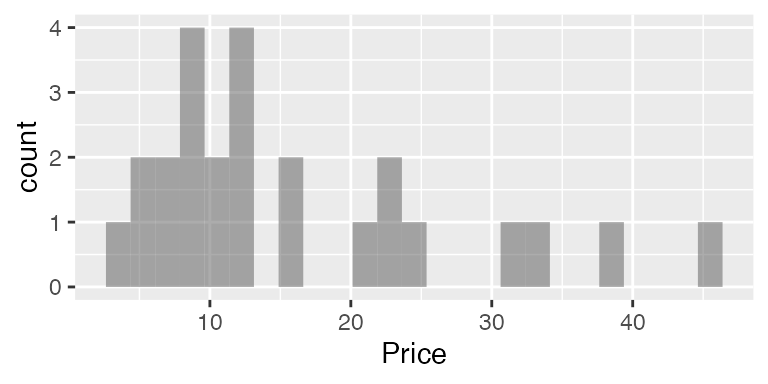
\includegraphics[width=\maxwidth]{figure/dot-1} 

}



\end{knitrout}

The basic \pkg{ggformula} syntax here --- operator, ``formula" involving \verb+~+, and the use of \texttt{data =} to specify the relevant data set --- will be used throughout \pkg{mosaic}.  For example, here is the sample mean 
\begin{knitrout}
\definecolor{shadecolor}{rgb}{0.969, 0.969, 0.969}\color{fgcolor}\begin{kframe}
\begin{alltt}
\hlkwd{mean}\hlstd{(}\hlopt{~} \hlstd{Price,} \hlkwc{data} \hlstd{= Mustangs)}
\end{alltt}
\begin{verbatim}
## [1] 16
\end{verbatim}
\end{kframe}
\end{knitrout}

Those familiar with \R{} may wonder why the statement has not been written as 
\begin{knitrout}
\definecolor{shadecolor}{rgb}{0.969, 0.969, 0.969}\color{fgcolor}\begin{kframe}
\begin{alltt}
\hlkwd{mean}\hlstd{(Mustangs}\hlopt{$}\hlstd{Price)}
\end{alltt}
\end{kframe}
\end{knitrout}
You can, of course, carry out exactly the same calculation this way.  By using 
\begin{knitrout}
\definecolor{shadecolor}{rgb}{0.969, 0.969, 0.969}\color{fgcolor}\begin{kframe}
\begin{alltt}
\hlkwd{mean}\hlstd{(}\hlopt{~} \hlstd{Price,} \hlkwc{data} \hlstd{= Mustangs)}
\end{alltt}
\end{kframe}
\end{knitrout}
we are making graphical and numerical summaries fit into a common template and 
anticipating the next steps, including the introduction of additional operations such as 
randomization and modeling.

Resampling, also known as random selection with replacement, is an important operation in randomization.  The \function{resample} function performs this.  It can be illustrated in a very basic way on a small set of numbers:
\begin{knitrout}
\definecolor{shadecolor}{rgb}{0.969, 0.969, 0.969}\color{fgcolor}\begin{kframe}
\begin{alltt}
\hlstd{simple} \hlkwb{=} \hlkwd{c}\hlstd{(}\hlnum{1}\hlstd{,} \hlnum{2}\hlstd{,} \hlnum{3}\hlstd{,} \hlnum{4}\hlstd{,} \hlnum{5}\hlstd{)}
\hlkwd{resample}\hlstd{(simple)}
\end{alltt}
\begin{verbatim}
## [1] 4 1 1 3 4
\end{verbatim}
\begin{alltt}
\hlkwd{resample}\hlstd{(simple)}
\end{alltt}
\begin{verbatim}
## [1] 4 3 3 4 1
\end{verbatim}
\begin{alltt}
\hlkwd{resample}\hlstd{(simple)}
\end{alltt}
\begin{verbatim}
## [1] 2 4 5 3 2
\end{verbatim}
\end{kframe}
\end{knitrout}

When applied to a dataframe, \function{resample} selects random rows.  It's easy to demonstrate this with a statement such as:

\begin{knitrout}
\definecolor{shadecolor}{rgb}{0.969, 0.969, 0.969}\color{fgcolor}\begin{kframe}
\begin{alltt}
\hlkwd{resample}\hlstd{(Mustangs)}
\end{alltt}
\end{kframe}
\end{knitrout}
\begin{knitrout}
\definecolor{shadecolor}{rgb}{0.969, 0.969, 0.969}\color{fgcolor}\begin{kframe}
\begin{verbatim}
##      Age Miles Price orig.id
## 13     8 100.8   9.0      13
## 3      9  82.8  11.9       3
## 2      7  33.0  45.0       2
## 24    12  72.9  12.9      24
## 2.1    7  33.0  45.0       2
## 24.1  12  72.9  12.9      24
## ... and so on
\end{verbatim}
\end{kframe}
\end{knitrout}

By reference to the case numbers in the left column, you can see that case 19 has been selected twice.

One resampling trial of the mean can be carried out with
\begin{knitrout}
\definecolor{shadecolor}{rgb}{0.969, 0.969, 0.969}\color{fgcolor}\begin{kframe}
\begin{alltt}
\hlkwd{mean}\hlstd{(}\hlopt{~} \hlstd{Price,} \hlkwc{data} \hlstd{=} \hlkwd{resample}\hlstd{(Mustangs))}
\end{alltt}
\begin{verbatim}
## [1] 16.3
\end{verbatim}
\end{kframe}
\end{knitrout}
Even though a single trial is of little use, it's a nice idea to have
students do the calculation to show that they are 
(usually) getting a different results with each resample.
  

Another trial can be carried out by repeating the command:
\begin{knitrout}
\definecolor{shadecolor}{rgb}{0.969, 0.969, 0.969}\color{fgcolor}\begin{kframe}
\begin{alltt}
\hlkwd{mean}\hlstd{(}\hlopt{~} \hlstd{Price,} \hlkwc{data} \hlstd{=} \hlkwd{resample}\hlstd{(Mustangs))}
\end{alltt}
\begin{verbatim}
## [1] 13.9
\end{verbatim}
\end{kframe}
\end{knitrout}
Let's generate five more, with a single command: 
\begin{knitrout}
\definecolor{shadecolor}{rgb}{0.969, 0.969, 0.969}\color{fgcolor}\begin{kframe}
\begin{alltt}
\hlkwd{do}\hlstd{(}\hlnum{5}\hlstd{)} \hlopt{*} \hlkwd{mean}\hlstd{(}\hlopt{~} \hlstd{Price,} \hlkwc{data} \hlstd{=} \hlkwd{resample}\hlstd{(Mustangs))}
\end{alltt}
\begin{verbatim}
##   mean
## 1 16.7
## 2 15.2
## 3 16.6
## 4 15.6
## 5 13.9
\end{verbatim}
\end{kframe}
\end{knitrout}
Now conduct 1000 resampling trials\footnote{1000 is a reasonable number of trials 
for illustration purposes, but Monte Carlo variability can be considerably reduced
by using 10,000 or more.
}, 
saving the results in an object
called \dataframe{Mustangs.Price.boot}:\footnote{It is a good idea to adopt a 
naming convention for your bootstrap and randomization distributions.  Repeatedly using
the same name (e.g., \texttt{Trials}) can become very confusing and lead to 
errors from misidentifying which distribution one has.  The name we have chosen here
makes it clear which data set an variable are being considered and that we are 
creating a bootstrap distribution (as opposed to simulating a null distribution).}
\begin{knitrout}
\definecolor{shadecolor}{rgb}{0.969, 0.969, 0.969}\color{fgcolor}\begin{kframe}
\begin{alltt}
\hlstd{Mustangs.Price.boot} \hlkwb{<-} \hlkwd{do}\hlstd{(}\hlnum{1000}\hlstd{)} \hlopt{*} \hlkwd{mean}\hlstd{(}\hlopt{~} \hlstd{Price,} \hlkwc{data} \hlstd{=} \hlkwd{resample}\hlstd{(Mustangs))}
\end{alltt}
\end{kframe}
\end{knitrout}


Plotting this resampling distribution is straightforward, e.g.:
\begin{knitrout}
\definecolor{shadecolor}{rgb}{0.969, 0.969, 0.969}\color{fgcolor}\begin{kframe}
\begin{alltt}
\hlkwd{gf_histogram}\hlstd{(}\hlopt{~} \hlstd{mean,} \hlkwc{data} \hlstd{= Mustangs.Price.boot,}
  \hlkwc{xlab}\hlstd{=}\hlstr{"Mean Mustang Price (in thousand dollars)"}\hlstd{)}
\end{alltt}
\end{kframe}

{\centering 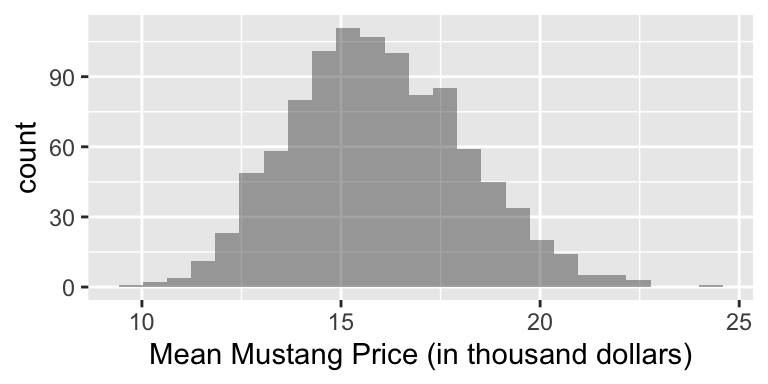
\includegraphics[width=\maxwidth]{figure/hist-1} 

}



\end{knitrout}

The simplest way to translate this distribution into a confidence interval is to apply the operator for that purpose:
\begin{knitrout}
\definecolor{shadecolor}{rgb}{0.969, 0.969, 0.969}\color{fgcolor}\begin{kframe}
\begin{alltt}
\hlkwd{confint}\hlstd{(Mustangs.Price.boot,} \hlkwc{level} \hlstd{=} \hlnum{0.90}\hlstd{,} \hlkwc{method} \hlstd{=} \hlstr{"quantile"}\hlstd{)}
\end{alltt}
\begin{verbatim}
##   name lower upper level     method estimate
## 1 mean  12.7  19.6   0.9 percentile       16
\end{verbatim}
\begin{alltt}
\hlkwd{confint}\hlstd{(Mustangs.Price.boot,} \hlkwc{level} \hlstd{=} \hlnum{0.90}\hlstd{,} \hlkwc{method} \hlstd{=} \hlstr{"stderr"}\hlstd{)}
\end{alltt}
\begin{verbatim}
##   name lower upper level method estimate margin.of.error df
## 1 mean  12.3  19.6   0.9 stderr       16            3.68 24
\end{verbatim}
\end{kframe}
\end{knitrout}
The \function{confint} function is a black box.  In introducing it, an instructor might well want to show the calculations behind the confidence interval in some detail using general-purpose operations.  \function{confint} implements two basic approaches, one based on quantiles of the distribution and the other using normal theory.
\begin{itemize}

\item Calculation of the 90\% confidence interval using quantiles
\begin{knitrout}
\definecolor{shadecolor}{rgb}{0.969, 0.969, 0.969}\color{fgcolor}\begin{kframe}
\begin{alltt}
\hlkwd{qdata}\hlstd{(}\hlopt{~} \hlstd{mean,} \hlkwd{c}\hlstd{(}\hlnum{.05}\hlstd{,} \hlnum{.95}\hlstd{),} \hlkwc{data} \hlstd{= Mustangs.Price.boot)}
\end{alltt}
\begin{verbatim}
##   5%  95% 
## 12.7 19.6
\end{verbatim}
\begin{alltt}
\hlcom{# alternative}
\hlkwd{cdata}\hlstd{(}\hlopt{~} \hlstd{mean,} \hlnum{0.90}\hlstd{,} \hlkwc{data} \hlstd{= Mustangs.Price.boot)}
\end{alltt}
\begin{verbatim}
##    lower upper central.p
## 5%  12.7  19.6       0.9
\end{verbatim}
\end{kframe}
\end{knitrout}

\item Using normal theory and the standard error.
First calculate the critical value $t_\star$ for
the appropriate degrees of freedom.  Or use $z_\star$, either for simplicity or to demonstrate how $t_\star$ differs.  In either case, the confidence level needs to be converted to the appropriate tail probability, e.g. a level of 90\% corresponds to a tail probability of 0.95.

\begin{knitrout}
\definecolor{shadecolor}{rgb}{0.969, 0.969, 0.969}\color{fgcolor}\begin{kframe}
\begin{alltt}
\hlstd{tstar} \hlkwb{<-} \hlkwd{qt}\hlstd{(}\hlnum{.95}\hlstd{,} \hlkwc{df} \hlstd{=} \hlnum{24}\hlstd{)}
\hlstd{zstar} \hlkwb{<-} \hlkwd{qnorm}\hlstd{(}\hlnum{.95}\hlstd{)}
\end{alltt}
\end{kframe}
\end{knitrout}
The resulting
margin of error will be
\begin{knitrout}
\definecolor{shadecolor}{rgb}{0.969, 0.969, 0.969}\color{fgcolor}\begin{kframe}
\begin{alltt}
\hlstd{tstar} \hlopt{*} \hlkwd{sd}\hlstd{(}\hlopt{~} \hlstd{mean,} \hlkwc{data} \hlstd{= Mustangs.Price.boot)}
\end{alltt}
\begin{verbatim}
## [1] 3.68
\end{verbatim}
\begin{alltt}
\hlstd{zstar} \hlopt{*} \hlkwd{sd}\hlstd{(}\hlopt{~} \hlstd{mean,} \hlkwc{data} \hlstd{= Mustangs.Price.boot)}
\end{alltt}
\begin{verbatim}
## [1] 3.54
\end{verbatim}
\end{kframe}
\end{knitrout}

\end{itemize}

There's little reason to repeat this set of commands every time one needs a confidence interval.  That's where \function{confint} comes in, abstracting the operation, allowing the user to specify a \texttt{level} and a \texttt{method} 
(\texttt{"quantile"} or \texttt{"stderr"}) and avoiding the need to convert the level into a tail probability.  The extent to which one should repeat the detailed steps of the margin-of-error calculation is a decision the instructor can make depending on local circumstances and the instructor's goals.  \R{} and \pkg{mosaic} supports both approaches.



\subsection*{Lock problem 2: Testing a proportion (NFL Overtimes)}

\begin{quotation}
{\em The National Football League (NFL) uses an overtime
period to determine a winner for games that are tied at the end of
regulation time.  The first team to score in the overtime wins the
game. A coin flip is used to determine which team gets the ball
first.  Is there an advantage to winning the coin flip?  Data from the
1974 through 2009 seasons show that the coin flip winner won 240 of
the 428 games where a winner was determined in overtime.  Treat these
as a sample of NFL games to test whether there is sufficient evidence
to show that the proportion of overtime games won by the coin flip
winner is more than one half.}
\end{quotation}

By and large, introductory students understand that, if first possession of the ball is unrelated to the game outcome, one would expect to see about half of the 428 games won by the team that won the coin flip.  The question is whether the observed 240 wins is ``about'' half of the 428 games.  Statistical inference compares the 240 to the $428/2 = 214$ in the context of sampling variation.

\paragraph{Style 1} Using the built-in binomial distribution operators.

Generate a simulation where each trial is a random sample of 428
games from a world in which the null hypothesis holds true and see what proportion of 
trials give a result as or more extreme as the observed 240.  

\begin{knitrout}
\definecolor{shadecolor}{rgb}{0.969, 0.969, 0.969}\color{fgcolor}\begin{kframe}
\begin{alltt}
\hlkwd{prop}\hlstd{(}\hlopt{~} \hlkwd{rbinom}\hlstd{(}\hlnum{1000}\hlstd{,} \hlkwc{prob} \hlstd{=} \hlnum{0.5}\hlstd{,} \hlkwc{size} \hlstd{=} \hlnum{428}\hlstd{)} \hlopt{>=} \hlnum{240}\hlstd{)}
\end{alltt}
\begin{verbatim}
## prop_TRUE 
##     0.007
\end{verbatim}
\end{kframe}
\end{knitrout}

The result indicates that it's very unlikely, if the null were true, that the coin flip winner would win 240 or more times.

The exact result differs slightly from one simulation to the next, but that variation can be made small by making the number of trials larger.

\begin{knitrout}
\definecolor{shadecolor}{rgb}{0.969, 0.969, 0.969}\color{fgcolor}\begin{kframe}
\begin{alltt}
\hlkwd{prop}\hlstd{(}\hlopt{~} \hlkwd{rbinom}\hlstd{(}\hlnum{1000}\hlstd{,} \hlkwc{prob} \hlstd{=} \hlnum{0.5}\hlstd{,} \hlkwc{size} \hlstd{=} \hlnum{428}\hlstd{)} \hlopt{>=} \hlnum{240}\hlstd{)}
\end{alltt}
\begin{verbatim}
## prop_TRUE 
##     0.004
\end{verbatim}
\end{kframe}
\end{knitrout}

In this case, it is 
tempting entirely to avoid the variation due to simulation by doing a deterministic
probability calculation rather than the simulation.  This exact reproducibility comes at
a cost, though, the need to customize the cut-off point to reflect which tail of the distribution corresponds to ``as or more extreme than 240."  On the right side, this means subtracting 1 from the observed number.
\begin{knitrout}
\definecolor{shadecolor}{rgb}{0.969, 0.969, 0.969}\color{fgcolor}\begin{kframe}
\begin{alltt}
\hlkwd{xpbinom}\hlstd{(}\hlnum{239}\hlstd{,} \hlkwc{prob} \hlstd{=} \hlnum{0.5}\hlstd{,} \hlkwc{size} \hlstd{=} \hlnum{428}\hlstd{)}
\end{alltt}
\begin{verbatim}
## [1] 0.993
\end{verbatim}
\end{kframe}

{\centering 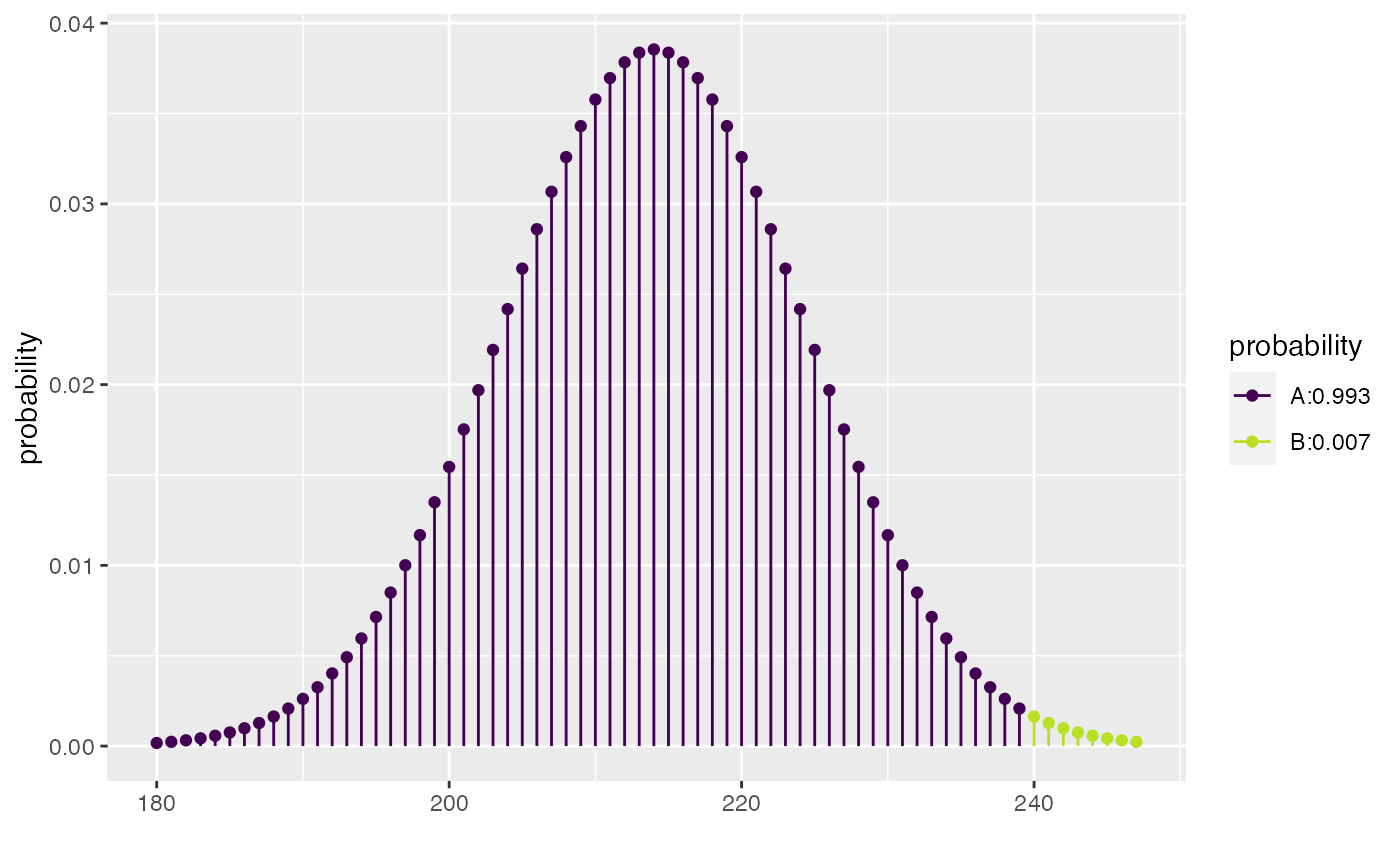
\includegraphics[width=\maxwidth]{figure/pbinom-1} 

}



\end{knitrout}

Of course, \R{} can handle all of these little details and do the entire 
calculation for us if we use the \function{binom.test} function.
\begin{knitrout}
\definecolor{shadecolor}{rgb}{0.969, 0.969, 0.969}\color{fgcolor}\begin{kframe}
\begin{alltt}
\hlkwd{binom.test}\hlstd{(}\hlkwc{x} \hlstd{=} \hlnum{240}\hlstd{,} \hlkwc{n} \hlstd{=} \hlnum{428}\hlstd{)}
\end{alltt}
\begin{verbatim}
## 
## 
## 
## data:  240 out of 428
## number of successes = 240, number of trials = 428, p-value =
## 0.01
## alternative hypothesis: true probability of success is not equal to 0.5
## 95 percent confidence interval:
##  0.512 0.608
## sample estimates:
## probability of success 
##                  0.561
\end{verbatim}
\end{kframe}
\end{knitrout}

Even if you want to use the deterministic probability calculation (using either
\function{pbinom} or \function{binom.test}), you might want to illustrate the logic with the random-number generator.

\paragraph{Style 2} Explicitly simulating a coin flip.

Recognizing that coin flips are a staple of statistics courses, the
\pkg{mosaic} package offers a function that simulates random coin tosses
without the need to refer to the binomial distribution.
Here is one trial involving flipping 428 coins:
\begin{knitrout}
\definecolor{shadecolor}{rgb}{0.969, 0.969, 0.969}\color{fgcolor}\begin{kframe}
\begin{alltt}
\hlkwd{do}\hlstd{(}\hlnum{1}\hlstd{)} \hlopt{*} \hlkwd{rflip}\hlstd{(}\hlnum{428}\hlstd{)}
\end{alltt}
\begin{verbatim}
##     n heads tails  prop
## 1 428   228   200 0.533
\end{verbatim}
\end{kframe}
\end{knitrout}

We'll do 1,000 trials, and count what fraction of the trials the
coin toss winner (say, ``heads'') wins 240 or more of the 428 attempts:
\begin{knitrout}
\definecolor{shadecolor}{rgb}{0.969, 0.969, 0.969}\color{fgcolor}\begin{kframe}
\begin{alltt}
\hlstd{NFL.null} \hlkwb{<-} \hlkwd{do}\hlstd{(}\hlnum{1000}\hlstd{)} \hlopt{*} \hlkwd{rflip}\hlstd{(}\hlnum{428}\hlstd{)}
\hlkwd{prop}\hlstd{(}\hlopt{~} \hlstd{heads} \hlopt{>=} \hlnum{240}\hlstd{,} \hlkwc{data} \hlstd{= NFL.null)}
\end{alltt}
\begin{verbatim}
## prop_TRUE 
##     0.005
\end{verbatim}
\end{kframe}
\end{knitrout}
\begin{knitrout}
\definecolor{shadecolor}{rgb}{0.969, 0.969, 0.969}\color{fgcolor}\begin{kframe}
\begin{alltt}
\hlkwd{gf_histogram}\hlstd{(}\hlopt{~} \hlstd{heads,} \hlkwc{fill} \hlstd{=} \hlopt{~} \hlstd{(heads} \hlopt{>=} \hlnum{240}\hlstd{),} \hlkwc{data} \hlstd{= NFL.null)}
\end{alltt}
\end{kframe}

{\centering 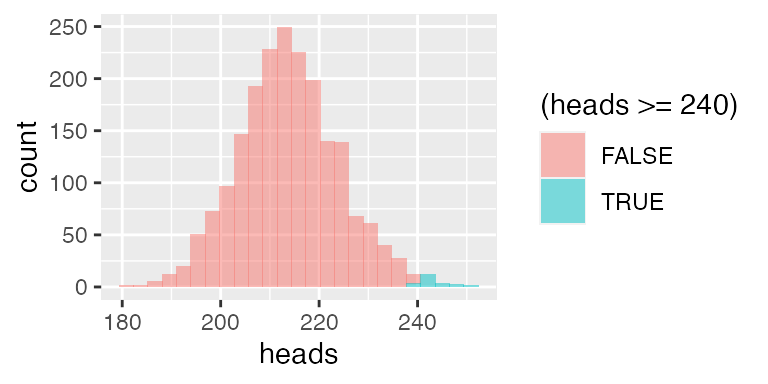
\includegraphics[width=\maxwidth]{figure/flips-1} 

}



\end{knitrout}

The observed pattern of 240 wins is not a likely outcome under the null hypothesis.
The shading added through the \option{groups =} option helps to visually reinforce the result.



\subsection*{Lock problem 3: Permutation test of means from two groups (sleep and memory)} 

\begin{quotation}
 {\em In an experiment on memory (Mednicj et al, 2008), students were given lists of 24 words
  to memorize.  After hearing the words they were assigned at random
  to different groups. One group of 12 students took a nap for 1.5
  hours while a second group of 12 students stayed awake and was given
  a caffeine pill.  The results below display the number of words each
  participant was able to recall after the break.  Test whether the
  data indicate a difference in mean number of words recalled between
  the two treatments.}
\end{quotation}
\begin{knitrout}
\definecolor{shadecolor}{rgb}{0.969, 0.969, 0.969}\color{fgcolor}\begin{kframe}
\begin{alltt}
\hlstd{Sleep} \hlkwb{<-} \hlkwd{read.csv}\hlstd{(}\hlstr{"http://www.mosaic-web.org/go/datasets/SleepCaffeine.csv"}\hlstd{)}
\end{alltt}
\end{kframe}
\end{knitrout}

The Sleep group tends to have remembered somewhat more words on average:
\begin{knitrout}
\definecolor{shadecolor}{rgb}{0.969, 0.969, 0.969}\color{fgcolor}\begin{kframe}
\begin{alltt}
\hlkwd{mean}\hlstd{(Words} \hlopt{~} \hlstd{Group,} \hlkwc{data} \hlstd{= Sleep)}
\end{alltt}
\begin{verbatim}
## Caffeine    Sleep 
##     12.2     15.2
\end{verbatim}
\begin{alltt}
\hlstd{obs} \hlkwb{<-} \hlkwd{diff}\hlstd{(}\hlkwd{mean}\hlstd{(Words} \hlopt{~} \hlstd{Group,} \hlkwc{data} \hlstd{= Sleep))}
\hlstd{obs}
\end{alltt}
\begin{verbatim}
## Sleep 
##     3
\end{verbatim}
\end{kframe}
\end{knitrout}

\begin{knitrout}
\definecolor{shadecolor}{rgb}{0.969, 0.969, 0.969}\color{fgcolor}\begin{kframe}
\begin{alltt}
\hlkwd{gf_boxplot}\hlstd{(Words} \hlopt{~} \hlstd{Group,} \hlkwc{data} \hlstd{= Sleep)}
\end{alltt}
\end{kframe}

{\centering 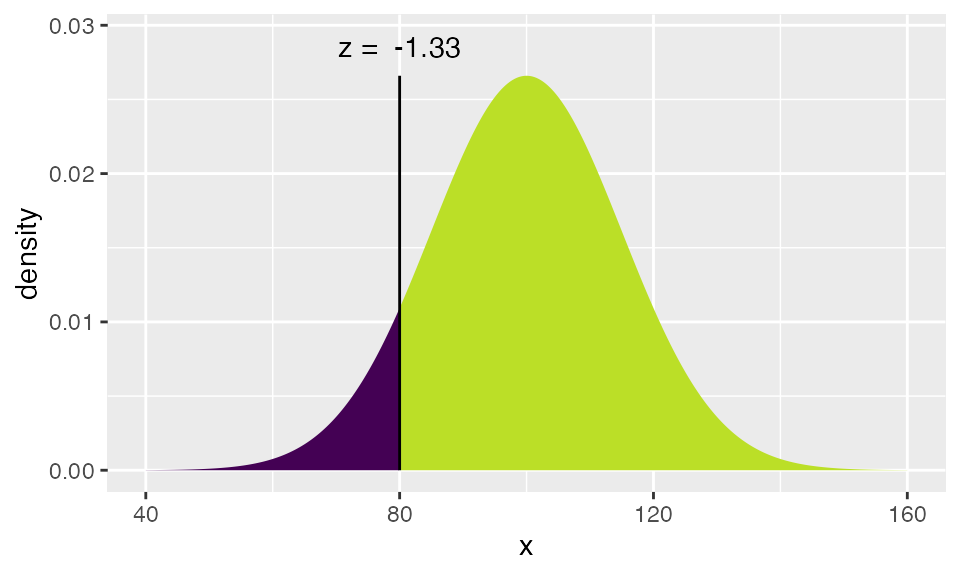
\includegraphics[width=\maxwidth]{figure/unnamed-chunk-13-1} 

}



\end{knitrout}

To implement the null hypothesis, scramble the Group with respect to the
outcome, Words:
\begin{knitrout}
\definecolor{shadecolor}{rgb}{0.969, 0.969, 0.969}\color{fgcolor}\begin{kframe}
\begin{alltt}
\hlkwd{diff}\hlstd{(}\hlkwd{mean}\hlstd{(Words} \hlopt{~} \hlkwd{shuffle}\hlstd{(Group),} \hlkwc{data} \hlstd{= Sleep))}
\end{alltt}
\begin{verbatim}
## Sleep 
## 0.167
\end{verbatim}
\end{kframe}
\end{knitrout}

That's just one trial.  Let's try again:
\begin{knitrout}
\definecolor{shadecolor}{rgb}{0.969, 0.969, 0.969}\color{fgcolor}\begin{kframe}
\begin{alltt}
\hlkwd{diff}\hlstd{(}\hlkwd{mean}\hlstd{(Words} \hlopt{~} \hlkwd{shuffle}\hlstd{(Group),} \hlkwc{data} \hlstd{= Sleep))}
\end{alltt}
\begin{verbatim}
## Sleep 
##     0
\end{verbatim}
\end{kframe}
\end{knitrout}
To get the distribution under the null
hypothesis, we carry out many trials:



\begin{knitrout}
\definecolor{shadecolor}{rgb}{0.969, 0.969, 0.969}\color{fgcolor}\begin{kframe}
\begin{alltt}
\hlstd{Sleep.null} \hlkwb{<-} \hlkwd{do}\hlstd{(}\hlnum{1000}\hlstd{)} \hlopt{*} \hlkwd{diff}\hlstd{(}\hlkwd{mean}\hlstd{(Words} \hlopt{~} \hlkwd{shuffle}\hlstd{(Group),} \hlkwc{data} \hlstd{= Sleep))}
\hlkwd{gf_histogram}\hlstd{(}\hlopt{~} \hlstd{Sleep,} \hlkwc{fill} \hlstd{=} \hlopt{~} \hlstd{(Sleep} \hlopt{>=} \hlstd{obs),} \hlkwc{data} \hlstd{= Sleep.null,}
  \hlkwc{binwidth} \hlstd{=} \hlnum{0.4}\hlstd{,}
  \hlkwc{xlab} \hlstd{=} \hlstr{"Distribution of difference in means\textbackslash{}nunder the null hypothesis"}\hlstd{)}
\end{alltt}
\end{kframe}

{\centering 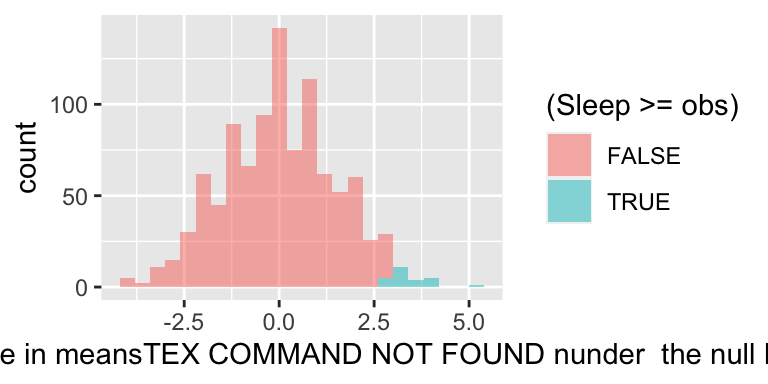
\includegraphics[width=\maxwidth]{figure/sleep-1} 

}



\end{knitrout}

The one-sided p-value for this test is the proportion of  
trials which yielded a result as extreme or more extreme as the observed difference.
We can calculate the one-sided p-value for this test by summing up the number of 
trials which yielded a result as extreme or more extreme as the observed difference.
Here only 27 of the 1000 trials gave a result that large, so the p-value is equal to 0.027.  We conclude that
it's unlikely that the two groups have the same mean word recall back in their respective populations.


\subsection*{Lock problem 4: Bootstrapping a correlation}

\begin{quotation}
{\em The data on Mustang prices in Problem \#1 also contains the number
 of miles each car had been driven (in thousands).  Find a
 95\% confidence interval for the correlation between price and mileage.}
\end{quotation}

We can fallow essentially the same workflow to obtain a confidence interval
for other statistics, including the correlation coefficient.\footnote{Naive 
confidence intervals based on percentiles or bootstrap standard errors from 
small samples may not be
as good as other methods (for example, the bootstrap t is preferred when
generating a confidence interval for a mean), and the ability to easily 
create simulated bootstrap distributions does not guarantee that the resulting
intervals will have the desired properties.  Alternative methods and diagnostics
are important topics not covered here.}
\begin{knitrout}
\definecolor{shadecolor}{rgb}{0.969, 0.969, 0.969}\color{fgcolor}\begin{kframe}
\begin{alltt}
\hlkwd{cor}\hlstd{(Price} \hlopt{~} \hlstd{Miles,} \hlkwc{data} \hlstd{= Mustangs)}
\end{alltt}
\begin{verbatim}
## [1] -0.825
\end{verbatim}
\end{kframe}
\end{knitrout}

\begin{knitrout}
\definecolor{shadecolor}{rgb}{0.969, 0.969, 0.969}\color{fgcolor}\begin{kframe}
\begin{alltt}
\hlstd{Mustangs.cor.boot} \hlkwb{<-} \hlkwd{do}\hlstd{(}\hlnum{1000}\hlstd{)} \hlopt{*} \hlkwd{cor}\hlstd{(Price} \hlopt{~} \hlstd{Miles,} \hlkwc{data} \hlstd{=} \hlkwd{resample}\hlstd{(Mustangs))}
\hlstd{quantiles} \hlkwb{<-} \hlkwd{qdata}\hlstd{(}\hlopt{~} \hlstd{cor,} \hlkwd{c}\hlstd{(}\hlnum{.025}\hlstd{,} \hlnum{.975}\hlstd{),} \hlkwc{data} \hlstd{= Mustangs.cor.boot)}
\hlstd{quantiles}
\end{alltt}
\begin{verbatim}
##   2.5%  97.5% 
## -0.928 -0.721
\end{verbatim}
\end{kframe}
\end{knitrout}

\begin{knitrout}
\definecolor{shadecolor}{rgb}{0.969, 0.969, 0.969}\color{fgcolor}\begin{kframe}
\begin{alltt}
\hlstd{Mustangs.hist} \hlkwb{<-} \hlkwd{mutate}\hlstd{(Mustangs.cor.boot,}
  \hlkwc{colorval} \hlstd{=} \hlkwd{cut}\hlstd{(cor,} \hlkwd{c}\hlstd{(}\hlopt{-}\hlnum{Inf}\hlstd{, quantiles,} \hlnum{Inf}\hlstd{),}
    \hlkwc{labels} \hlstd{=} \hlkwd{c}\hlstd{(}\hlstr{"Lower"}\hlstd{,} \hlstr{"Middle"}\hlstd{,} \hlstr{"Upper"}\hlstd{)))}
\hlkwd{gf_histogram}\hlstd{(}\hlopt{~} \hlstd{cor,} \hlkwc{data} \hlstd{= Mustangs.hist,} \hlkwc{fill} \hlstd{=} \hlopt{~} \hlstd{colorval,} \hlkwc{n} \hlstd{=} \hlnum{50}\hlstd{)}
\hlkwd{confint}\hlstd{(Mustangs.cor.boot)}
\end{alltt}
\begin{verbatim}
##   name  lower  upper level     method estimate
## 1  cor -0.928 -0.721  0.95 percentile   -0.825
\end{verbatim}
\end{kframe}

{\centering 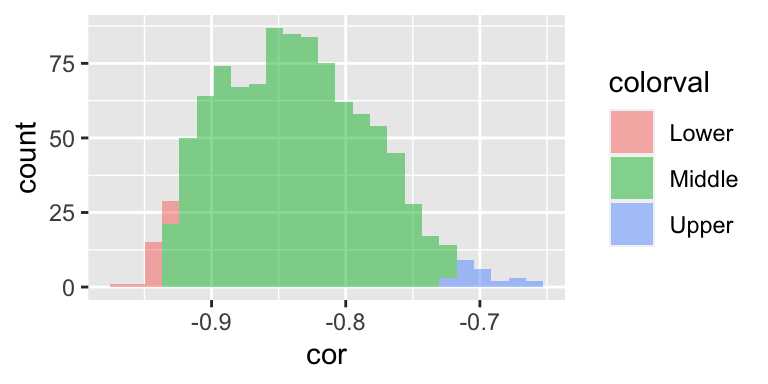
\includegraphics[width=\maxwidth]{figure/cor-1} 

}



\end{knitrout}





\section{Moving beyond means and proportions}

The Lock problems refer to the descriptive statistics encountered in many 
introductory applied statistics courses: 
means, proportions, differences in means and proportions. There are advantages, however, 
in introducing such basic statistics in the context of a more general framework: 
linear models.  

Usually, people think about linear models in the context of regression.  For instance, using the Lock Mustang price dataset, 
there is presumably a relationship between the price of a car and its mileage.  Here's a graph:

\begin{knitrout}
\definecolor{shadecolor}{rgb}{0.969, 0.969, 0.969}\color{fgcolor}\begin{kframe}
\begin{alltt}
\hlkwd{gf_point}\hlstd{(Price} \hlopt{~} \hlstd{Miles,} \hlkwc{data} \hlstd{= Mustangs)} \hlopt
  \hlkwd{gf_lm}\hlstd{()}
\end{alltt}
\end{kframe}

{\centering 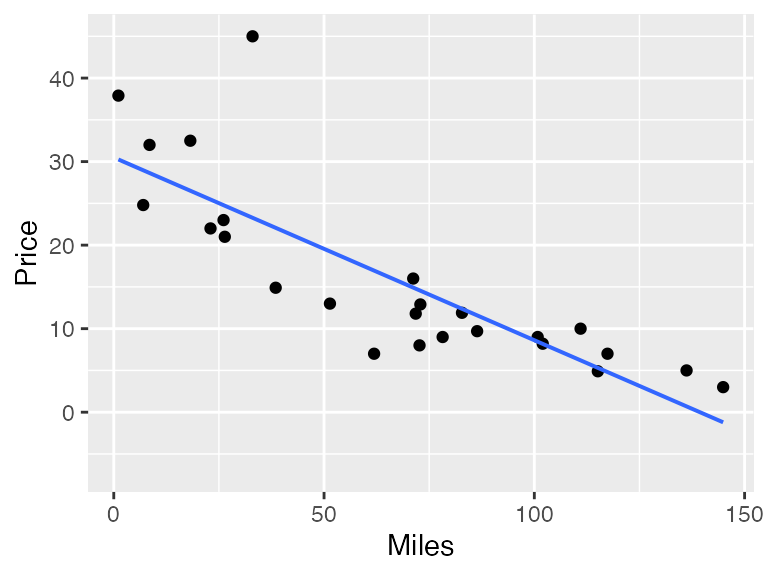
\includegraphics[width=\maxwidth]{figure/price-mileage-graph-1} 

}



\end{knitrout}
There's a pretty clear relationship here, which in the Lock problems was quantified with the correlation coefficient.

In regression, one finds a straight-line functional relationship between the two variables.
The built-in \R{} \function{lm} function does the calculations:
\begin{knitrout}
\definecolor{shadecolor}{rgb}{0.969, 0.969, 0.969}\color{fgcolor}\begin{kframe}
\begin{alltt}
\hlkwd{lm}\hlstd{(Price} \hlopt{~} \hlstd{Miles,} \hlkwc{data} \hlstd{= Mustangs)}
\end{alltt}
\begin{verbatim}
## 
## Call:
## lm(formula = Price ~ Miles, data = Mustangs)
## 
## Coefficients:
## (Intercept)        Miles  
##      30.495       -0.219
\end{verbatim}
\end{kframe}
\end{knitrout}
The notation used is the same as used to produce a scatter plot.  
The result indicates that for every additional 1000 miles driven, the price of a car 
typically decreases by \$219 dollars (or, given the units of the data, 0.2188 thousand 
dollars).  In other words, the value of a Mustang goes down by about 22 cents per mile 
driven.

This number, 22 cents decrease per mile, can be thought of as an ``effect size.''  It's likely much more meaningful to students (and car buyers!) than the correlation coefficient of $-0.82$.  The ability to give a description in terms of an effect size is an advantage of using regression as a description rather than correlation.  There are more such advantages to regression, which we will describe later.  But for now, our emphasis is on the use of regression as a framework for the traditional sorts of calculations of means, proportions, and differences of means and proportions.

The mean price of the Mustangs is, calculated in the ordinary way:
\begin{knitrout}
\definecolor{shadecolor}{rgb}{0.969, 0.969, 0.969}\color{fgcolor}\begin{kframe}
\begin{alltt}
\hlkwd{mean}\hlstd{(}\hlopt{~} \hlstd{Price,} \hlkwc{data} \hlstd{= Mustangs)}
\end{alltt}
\begin{verbatim}
## [1] 16
\end{verbatim}
\end{kframe}
\end{knitrout}

The same result can be generate via a linear model:
\begin{knitrout}
\definecolor{shadecolor}{rgb}{0.969, 0.969, 0.969}\color{fgcolor}\begin{kframe}
\begin{alltt}
\hlkwd{lm}\hlstd{(Price} \hlopt{~} \hlnum{1}\hlstd{,} \hlkwc{data} \hlstd{= Mustangs)}
\end{alltt}
\begin{verbatim}
## 
## Call:
## lm(formula = Price ~ 1, data = Mustangs)
## 
## Coefficients:
## (Intercept)  
##          16
\end{verbatim}
\end{kframe}
\end{knitrout}

This may seem obscure.  In \function{lm}, the \verb+~+ notation is used to identify the
response variable and the explanatory variables.  In \verb+Price ~ Miles+, the response variable is \texttt{Price} and \texttt{Miles} is being used as the explanatory variable.  
The mileage varies from car to car; this variation in mileage is used to explain the variation in price.

In \verb+Price ~ 1+, the \texttt{1} can be thought of as signifying that there are no explanatory variables, or, from a slightly different perspective, that the cars are all the same. The \function{mean} function is set up to accept this same notation:
\begin{knitrout}
\definecolor{shadecolor}{rgb}{0.969, 0.969, 0.969}\color{fgcolor}\begin{kframe}
\begin{alltt}
\hlkwd{mean}\hlstd{(Price} \hlopt{~} \hlnum{1}\hlstd{,} \hlkwc{data} \hlstd{= Mustangs)}
\end{alltt}
\begin{verbatim}
##  1 
## 16
\end{verbatim}
\end{kframe}
\end{knitrout}
Why?  So that the notation can be extended to include calculating the mean for different groups.  To illustrate, consider the Lock \texttt{Sleep} data which compares the ability to memorize words after a nap versus after taking caffeine.

The mean number of words memorized, ignoring the explanatory group, is:
\begin{knitrout}
\definecolor{shadecolor}{rgb}{0.969, 0.969, 0.969}\color{fgcolor}\begin{kframe}
\begin{alltt}
\hlkwd{mean}\hlstd{(Words} \hlopt{~} \hlnum{1}\hlstd{,} \hlkwc{data} \hlstd{= Sleep)}
\end{alltt}
\begin{verbatim}
##    1 
## 13.8
\end{verbatim}
\end{kframe}
\end{knitrout}
To break this down by groups, use an explanatory variable:
\begin{knitrout}
\definecolor{shadecolor}{rgb}{0.969, 0.969, 0.969}\color{fgcolor}\begin{kframe}
\begin{alltt}
\hlkwd{mean}\hlstd{(Words} \hlopt{~} \hlstd{Group,} \hlkwc{data} \hlstd{= Sleep)}
\end{alltt}
\begin{verbatim}
## Caffeine    Sleep 
##     12.2     15.2
\end{verbatim}
\end{kframe}
\end{knitrout}

Conventionally, regression is introduced as a technique for working with quantitative explanatory variables, e.g. the \texttt{Miles} in the Mustang data, while groupwise means are used for categorical variables such as \texttt{Group} in the sleep data.  But the regression technique applies to categorical data as well:
\begin{knitrout}
\definecolor{shadecolor}{rgb}{0.969, 0.969, 0.969}\color{fgcolor}\begin{kframe}
\begin{alltt}
\hlkwd{lm}\hlstd{(Words} \hlopt{~} \hlstd{Group,} \hlkwc{data} \hlstd{= Sleep)}
\end{alltt}
\begin{verbatim}
## 
## Call:
## lm(formula = Words ~ Group, data = Sleep)
## 
## Coefficients:
## (Intercept)   GroupSleep  
##        12.2          3.0
\end{verbatim}
\end{kframe}
\end{knitrout}
What's different between the information reported from \function{mean} and the result of \function{lm} is the format of the results.  The \texttt{GroupSleep} coefficient from \function{lm} gives the {\em difference} between the two groups.
\begin{knitrout}
\definecolor{shadecolor}{rgb}{0.969, 0.969, 0.969}\color{fgcolor}\begin{kframe}
\begin{alltt}
\hlkwd{diffmean}\hlstd{(Words} \hlopt{~} \hlstd{Group,} \hlkwc{data} \hlstd{= Sleep)}
\end{alltt}
\begin{verbatim}
## diffmean 
##        3
\end{verbatim}
\end{kframe}
\end{knitrout}

The \function{lm} function also can be used to calculate proportions and differences in proportions.  We'll illustrate with the \texttt{HELPrct} data which contains information about patients in the Health Evaluation and Linkage to Primary Care randomized clinical trial.  Consider the proportion of people who are reported as homeless:
\begin{knitrout}
\definecolor{shadecolor}{rgb}{0.969, 0.969, 0.969}\color{fgcolor}\begin{kframe}
\begin{alltt}
\hlkwd{prop}\hlstd{(homeless} \hlopt{~} \hlnum{1}\hlstd{,} \hlkwc{data} \hlstd{= HELPrct)}
\end{alltt}
\begin{verbatim}
## prop_homeless.1 
##           0.461
\end{verbatim}
\end{kframe}
\end{knitrout}

The proportion of patients who are homeless differs somewhat between the sexes; males are somewhat more likely to be homeless.
\begin{knitrout}
\definecolor{shadecolor}{rgb}{0.969, 0.969, 0.969}\color{fgcolor}\begin{kframe}
\begin{alltt}
\hlkwd{prop}\hlstd{(homeless} \hlopt{~} \hlstd{sex,} \hlkwc{data} \hlstd{= HELPrct)}
\end{alltt}
\begin{verbatim}
## prop_homeless.female   prop_homeless.male 
##                0.374                0.488
\end{verbatim}
\end{kframe}
\end{knitrout}

The difference between these two proportions is:
\begin{knitrout}
\definecolor{shadecolor}{rgb}{0.969, 0.969, 0.969}\color{fgcolor}\begin{kframe}
\begin{alltt}
\hlkwd{diffprop}\hlstd{(homeless} \hlopt{~} \hlstd{sex,} \hlkwc{data} \hlstd{= HELPrct)}
\end{alltt}
\begin{verbatim}
## diffprop 
##    0.115
\end{verbatim}
\end{kframe}
\end{knitrout}

The \texttt{lm} function gives the same results. (You have to specify which level you want the proportion of, ``homeless" or ``housed".)
\begin{knitrout}
\definecolor{shadecolor}{rgb}{0.969, 0.969, 0.969}\color{fgcolor}\begin{kframe}
\begin{alltt}
\hlkwd{lm}\hlstd{(homeless}\hlopt{==}\hlstr{"homeless"} \hlopt{~} \hlnum{1}\hlstd{,} \hlkwc{data} \hlstd{= HELPrct)}
\end{alltt}
\begin{verbatim}
## 
## Call:
## lm(formula = homeless == "homeless" ~ 1, data = HELPrct)
## 
## Coefficients:
## (Intercept)  
##       0.461
\end{verbatim}
\end{kframe}
\end{knitrout}

Why use \function{lm} when \function{mean} and \function{prop} and 
(and \function{diffmean} and \function{diffprop}) will give the same result?  
Because \function{lm} can be generalized.  It works for both categorical and 
quantitative explanatory variables and, very importantly, \function{lm} 
allows multiple explanatory variables to be used.

Even when using \function{mean} and \function{prop}, there's a reason to prefer the \verb+~1+ notation.  It emphasizes that the calculation is not trying to explain the variability in the response variable; there are no explanatory variables being used.  


\begin{knitrout}
\definecolor{shadecolor}{rgb}{0.969, 0.969, 0.969}\color{fgcolor}\begin{kframe}
\begin{alltt}
\hlkwd{lm}\hlstd{(homeless}\hlopt{==}\hlstr{"homeless"} \hlopt{~} \hlstd{sex,} \hlkwc{data} \hlstd{= HELPrct)}
\end{alltt}
\begin{verbatim}
## 
## Call:
## lm(formula = homeless == "homeless" ~ sex, data = HELPrct)
## 
## Coefficients:
## (Intercept)      sexmale  
##       0.374        0.115
\end{verbatim}
\end{kframe}
\end{knitrout}

\subsection{Randomization with linear models}

Randomization can be performed with \function{lm} in the same style as with \function{mean} and \function{prop}.  Here, for instance, is a resampling confidence interval on the 
price change with mileage in the Mustang data:
\begin{knitrout}
\definecolor{shadecolor}{rgb}{0.969, 0.969, 0.969}\color{fgcolor}\begin{kframe}
\begin{alltt}
\hlstd{Mustangs.lm.boot} \hlkwb{<-} \hlkwd{do}\hlstd{(}\hlnum{1000}\hlstd{)} \hlopt{*} \hlkwd{lm}\hlstd{(Price} \hlopt{~} \hlstd{Miles,} \hlkwc{data} \hlstd{=} \hlkwd{resample}\hlstd{(Mustangs))}
\hlkwd{confint}\hlstd{(Mustangs.lm.boot)}
\end{alltt}
\begin{verbatim}
##        name  lower   upper level     method estimate
## 1 Intercept 24.112  35.755  0.95 percentile   30.495
## 2     Miles -0.277  -0.159  0.95 percentile   -0.219
## 3     sigma  3.234   8.923  0.95 percentile    6.422
## 4 r.squared  0.520   0.864  0.95 percentile    0.680
## 5         F 24.957 146.387  0.95 percentile   48.873
\end{verbatim}
\end{kframe}
\end{knitrout}


Or, we can calculate a permutation test on the difference between homeless rates among men and women using the \texttt{HELPrct} data:

\begin{knitrout}
\definecolor{shadecolor}{rgb}{0.969, 0.969, 0.969}\color{fgcolor}\begin{kframe}
\begin{alltt}
\hlstd{HELPrct.null} \hlkwb{<-} \hlkwd{do}\hlstd{(}\hlnum{1000}\hlstd{)} \hlopt{*} \hlkwd{lm}\hlstd{(homeless}\hlopt{==}\hlstr{"homeless"} \hlopt{~} \hlkwd{shuffle}\hlstd{(sex),} \hlkwc{data} \hlstd{= HELPrct)}
\hlkwd{prop}\hlstd{(}\hlopt{~} \hlstd{(}\hlkwd{abs}\hlstd{(sexmale)} \hlopt{>} \hlnum{0.1146}\hlstd{),} \hlkwc{data} \hlstd{= HELPrct.null)}
\end{alltt}
\begin{verbatim}
## prop_TRUE 
##     0.044
\end{verbatim}
\end{kframe}
\end{knitrout}

\subsection{Multiple explanatory variables}

The regression framework allows more than one explanatory to be used.  For instance, one can examine how each of \texttt{Age} and \texttt{Miles} is related to the \texttt{Price} of the Mustangs.

\begin{knitrout}
\definecolor{shadecolor}{rgb}{0.969, 0.969, 0.969}\color{fgcolor}\begin{kframe}
\begin{alltt}
\hlstd{Mustangs.boot1} \hlkwb{<-} \hlkwd{do}\hlstd{(}\hlnum{1000}\hlstd{)} \hlopt{*} \hlkwd{lm}\hlstd{(Price} \hlopt{~} \hlstd{Age,} \hlkwc{data} \hlstd{=} \hlkwd{resample}\hlstd{(Mustangs))}
\hlstd{Mustangs.boot2} \hlkwb{<-} \hlkwd{do}\hlstd{(}\hlnum{1000}\hlstd{)} \hlopt{*} \hlkwd{lm}\hlstd{(Price} \hlopt{~} \hlstd{Miles,} \hlkwc{data} \hlstd{=} \hlkwd{resample}\hlstd{(Mustangs))}
\hlstd{Mustangs.boot3} \hlkwb{<-} \hlkwd{do}\hlstd{(}\hlnum{1000}\hlstd{)} \hlopt{*} \hlkwd{lm}\hlstd{(Price} \hlopt{~} \hlstd{Miles} \hlopt{+} \hlstd{Age,} \hlkwc{data} \hlstd{=} \hlkwd{resample}\hlstd{(Mustangs))}
\end{alltt}
\end{kframe}
\end{knitrout}
The first model suggests that \texttt{Price} goes down by about one to two thousand dollars per year of \texttt{Age}. 

\begin{knitrout}
\definecolor{shadecolor}{rgb}{0.969, 0.969, 0.969}\color{fgcolor}\begin{kframe}
\begin{alltt}
\hlkwd{confint}\hlstd{(Mustangs.boot1)}
\end{alltt}
\begin{verbatim}
##        name  lower  upper level     method estimate
## 1 Intercept 23.981 37.673  0.95 percentile   30.264
## 2       Age -2.355 -1.213  0.95 percentile   -1.717
## 3     sigma  4.247 11.218  0.95 percentile    8.102
## 4 r.squared  0.281  0.751  0.95 percentile    0.491
## 5         F  8.982 69.529  0.95 percentile   22.154
\end{verbatim}
\end{kframe}
\end{knitrout}
The second model indicates that \texttt{Price} goes down by about 16 to 28 cents per mile driven.
\begin{knitrout}
\definecolor{shadecolor}{rgb}{0.969, 0.969, 0.969}\color{fgcolor}\begin{kframe}
\begin{alltt}
\hlkwd{confint}\hlstd{(Mustangs.boot2)}
\end{alltt}
\begin{verbatim}
##        name  lower   upper level     method estimate
## 1 Intercept 24.095  35.871  0.95 percentile   30.495
## 2     Miles -0.277  -0.158  0.95 percentile   -0.219
## 3     sigma  3.020   8.838  0.95 percentile    6.422
## 4 r.squared  0.529   0.855  0.95 percentile    0.680
## 5         F 25.796 135.855  0.95 percentile   48.873
\end{verbatim}
\end{kframe}
\end{knitrout}

The third model puts each explanatory variable in the context of the other, and suggests that \texttt{Age} may just be a proxy for \texttt{Miles}.
\begin{knitrout}
\definecolor{shadecolor}{rgb}{0.969, 0.969, 0.969}\color{fgcolor}\begin{kframe}
\begin{alltt}
\hlkwd{confint}\hlstd{(Mustangs.boot3)}
\end{alltt}
\begin{verbatim}
##        name  lower  upper level     method estimate
## 1 Intercept 25.751 36.315  0.95 percentile   30.867
## 2     Miles -0.339 -0.110  0.95 percentile   -0.205
## 3       Age -0.838  0.874  0.95 percentile   -0.155
## 4     sigma  3.047  9.023  0.95 percentile    6.553
## 5 r.squared  0.537  0.879  0.95 percentile    0.681
## 6         F 12.754 80.145  0.95 percentile   23.512
\end{verbatim}
\end{kframe}
\end{knitrout}
One way to interpret this result is that, adjusting for \texttt{Miles}, 
there is little 
evidence for an \texttt{Age} effect.  The inflation of the confidence intervals for 
\texttt{Miles} and \texttt{Age} is a result of the collinearity 
between those explanatory variables. 

\subsection{Simulation and {\sc ANOVA}}

One way to think about {\sc ANOVA} is a way of quantifying the extent to which a model term, in the context of other model terms, is better than random ``junk.'' Consider, for example, the role of \texttt{Age} in a model of the Mustang prices that includes \texttt{Miles}.  Here's one {\sc ANOVA} report:
\begin{knitrout}
\definecolor{shadecolor}{rgb}{0.969, 0.969, 0.969}\color{fgcolor}\begin{kframe}
\begin{alltt}
\hlkwd{anova}\hlstd{(}\hlkwd{lm}\hlstd{(Price} \hlopt{~} \hlstd{Miles} \hlopt{+} \hlstd{Age,} \hlkwc{data} \hlstd{= Mustangs))}
\end{alltt}
\begin{verbatim}
## Analysis of Variance Table
## 
## Response: Price
##           Df Sum Sq Mean Sq F value Pr(>F)    
## Miles      1   2016    2016   46.94  7e-07 ***
## Age        1      4       4    0.09   0.77    
## Residuals 22    945      43                   
## ---
## Signif. codes:  0 '***' 0.001 '**' 0.01 '*' 0.05 '.' 0.1 ' ' 1
\end{verbatim}
\end{kframe}
\end{knitrout}
The p-value on \texttt{Age} suggests that \texttt{Age} is not contributing to the model.  But there's a different {\sc ANOVA} report available that suggests a different conclusion.
\begin{knitrout}
\definecolor{shadecolor}{rgb}{0.969, 0.969, 0.969}\color{fgcolor}\begin{kframe}
\begin{alltt}
\hlkwd{anova}\hlstd{(}\hlkwd{lm}\hlstd{(Price} \hlopt{~} \hlstd{Age} \hlopt{+} \hlstd{Miles,} \hlkwc{data} \hlstd{= Mustangs))}
\end{alltt}
\begin{verbatim}
## Analysis of Variance Table
## 
## Response: Price
##           Df Sum Sq Mean Sq F value  Pr(>F)    
## Age        1   1454    1454    33.9 7.4e-06 ***
## Miles      1    565     565    13.2  0.0015 ** 
## Residuals 22    945      43                    
## ---
## Signif. codes:  0 '***' 0.001 '**' 0.01 '*' 0.05 '.' 0.1 ' ' 1
\end{verbatim}
\end{kframe}
\end{knitrout}
The difference between the two {\sc ANOVA} reports can be explained in 
several ways, for example by regarding {\sc ANOVA} as a sequential report 
on a nested sequence of models, so that the order of model terms makes 
a difference.  For instance, the $R^2$ from this sequence of models suggests 
that \texttt{Age} doesn't add much to \texttt{Miles}.

\begin{knitrout}
\definecolor{shadecolor}{rgb}{0.969, 0.969, 0.969}\color{fgcolor}\begin{kframe}
\begin{alltt}
\hlkwd{do}\hlstd{(}\hlnum{1}\hlstd{)} \hlopt{*} \hlkwd{lm}\hlstd{(Price} \hlopt{~} \hlstd{Miles,} \hlkwc{data} \hlstd{= Mustangs)}
\end{alltt}
\begin{verbatim}
##   Intercept  Miles sigma r.squared    F numdf dendf .row .index
## 1      30.5 -0.219  6.42      0.68 48.9     1    23    1      1
\end{verbatim}
\begin{alltt}
\hlkwd{do}\hlstd{(}\hlnum{1}\hlstd{)} \hlopt{*} \hlkwd{lm}\hlstd{(Price} \hlopt{~} \hlstd{Miles} \hlopt{+} \hlstd{Age,} \hlkwc{data} \hlstd{= Mustangs)}
\end{alltt}
\begin{verbatim}
##   Intercept  Miles    Age sigma r.squared    F numdf dendf .row
## 1      30.9 -0.205 -0.155  6.55     0.681 23.5     2    22    1
##   .index
## 1      1
\end{verbatim}
\end{kframe}
\end{knitrout}

Here, \function{do} has been used without any randomization, merely to format the results in a way that allows them be readily compared.  Note that the addition of \texttt{Age} as an explanatory variable has increased $R^2$ by a little bit, from $0.680$ to $0.681$.  

Shuffling \texttt{Age} allows the actual change in $R^2$ to be compared to what would be expected under the null hypothesis:
\begin{knitrout}
\definecolor{shadecolor}{rgb}{0.969, 0.969, 0.969}\color{fgcolor}\begin{kframe}
\begin{alltt}
\hlstd{Mustangs.Age.boot} \hlkwb{<-} \hlkwd{do}\hlstd{(}\hlnum{1000}\hlstd{)} \hlopt{*} \hlkwd{lm}\hlstd{(Price} \hlopt{~} \hlstd{Miles} \hlopt{+} \hlkwd{shuffle}\hlstd{(Age),} \hlkwc{data} \hlstd{= Mustangs )}
\hlkwd{favstats}\hlstd{(}\hlopt{~} \hlstd{r.squared,} \hlkwc{data} \hlstd{= Mustangs.Age.boot)}
\end{alltt}
\begin{verbatim}
##   min    Q1 median    Q3   max  mean     sd    n missing
##  0.68 0.682  0.687 0.699 0.803 0.694 0.0169 1000       0
\end{verbatim}
\begin{alltt}
\hlkwd{cdata}\hlstd{(}\hlopt{~} \hlstd{r.squared,} \hlnum{.95}\hlstd{,} \hlkwc{data} \hlstd{= Mustangs.Age.boot)}
\end{alltt}
\begin{verbatim}
##      lower upper central.p
## 2.5%  0.68 0.738      0.95
\end{verbatim}
\end{kframe}
\end{knitrout}

The observed $R^2$ from \verb-Price ~ Miles + Age- falls in the middle portion of the 
observed range when \texttt{Age} is shuffled.  We can conclude that \texttt{Age} is not an important predictor.

The result is very different when \texttt{Miles} is shuffled instead.
\begin{knitrout}
\definecolor{shadecolor}{rgb}{0.969, 0.969, 0.969}\color{fgcolor}\begin{kframe}
\begin{alltt}
\hlstd{Mustangs.Miles.boot} \hlkwb{<-} \hlkwd{do}\hlstd{(}\hlnum{1000}\hlstd{)} \hlopt{*} \hlkwd{lm}\hlstd{(Price} \hlopt{~} \hlkwd{shuffle}\hlstd{(Miles)} \hlopt{+} \hlstd{Age,} \hlkwc{data} \hlstd{= Mustangs)}
\hlkwd{favstats}\hlstd{(}\hlopt{~} \hlstd{r.squared,} \hlkwc{data} \hlstd{= Mustangs.Miles.boot)}
\end{alltt}
\begin{verbatim}
##    min    Q1 median    Q3   max  mean    sd    n missing
##  0.491 0.493  0.502 0.523 0.718 0.513 0.029 1000       0
\end{verbatim}
\begin{alltt}
\hlkwd{cdata}\hlstd{(}\hlopt{~} \hlstd{r.squared,} \hlnum{.95}\hlstd{,} \hlkwc{data} \hlstd{= Mustangs.Miles.boot)}
\end{alltt}
\begin{verbatim}
##      lower upper central.p
## 2.5% 0.491 0.594      0.95
\end{verbatim}
\end{kframe}
\end{knitrout}
The observed value of $R^2 = 0.681$ falls well above the central 95\% of resampled values: 
we conclude that  \texttt{Miles} is an important predictor.

\section{Using simulations in other ways}

The basic technology of resampling and shuffling can be used to
demonstrate many other concepts in statistics than the generation of
confidence intervals and p-values.  For example, it is very useful for
showing the origins of distributions such as t and F.  

For the sake of illustration, consider a $\chi^2$-test of the independence of \texttt{homeless} and \texttt{sex} in the \texttt{HELPrct} data.
To illustrate, here is a simulation to construct the distribution of p-values from a simple test under the null hypothesis.  The 

\begin{enumerate}
\item Carry out the test, e.g.
\begin{knitrout}
\definecolor{shadecolor}{rgb}{0.969, 0.969, 0.969}\color{fgcolor}\begin{kframe}
\begin{alltt}
\hlkwd{chisq.test}\hlstd{(}\hlkwd{tally}\hlstd{(}\hlopt{~} \hlstd{homeless} \hlopt{+} \hlstd{sex,}
                   \hlkwc{data} \hlstd{= HELPrct,} \hlkwc{margins} \hlstd{=} \hlnum{FALSE}\hlstd{))}
\end{alltt}
\begin{verbatim}
## 
## 	Pearson's Chi-squared test with Yates' continuity correction
## 
## data:  tally(~homeless + sex, data = HELPrct, margins = FALSE)
## X-squared = 4, df = 1, p-value = 0.05
\end{verbatim}
\end{kframe}
\end{knitrout}

\item Modify the statement to extract the portion of interest.  
In this case, the p-value:
\begin{knitrout}
\definecolor{shadecolor}{rgb}{0.969, 0.969, 0.969}\color{fgcolor}\begin{kframe}
\begin{alltt}
\hlkwd{pval}\hlstd{(}\hlkwd{chisq.test}\hlstd{(}\hlkwd{tally}\hlstd{(}\hlopt{~} \hlstd{homeless} \hlopt{+} \hlstd{sex,}
                   \hlkwc{data} \hlstd{= HELPrct,} \hlkwc{margins} \hlstd{=} \hlnum{FALSE}\hlstd{)) )}
\end{alltt}
\begin{verbatim}
## p.value 
##  0.0491
\end{verbatim}
\end{kframe}
\end{knitrout}

\item Insert randomization to implement the null hypothesis:
\begin{knitrout}
\definecolor{shadecolor}{rgb}{0.969, 0.969, 0.969}\color{fgcolor}\begin{kframe}
\begin{alltt}
\hlkwd{pval}\hlstd{(}\hlkwd{chisq.test}\hlstd{(}\hlkwd{tally}\hlstd{(}\hlopt{~} \hlkwd{shuffle}\hlstd{(homeless)} \hlopt{+} \hlstd{sex,}
                         \hlkwc{data} \hlstd{= HELPrct,} \hlkwc{margins} \hlstd{=} \hlnum{FALSE}\hlstd{)))}
\end{alltt}
\begin{verbatim}
## p.value 
##       1
\end{verbatim}
\end{kframe}
\end{knitrout}

\item Iterate to get the distribution under the null:
\begin{knitrout}
\definecolor{shadecolor}{rgb}{0.969, 0.969, 0.969}\color{fgcolor}\begin{kframe}
\begin{alltt}
\hlstd{Chisq.null} \hlkwb{<-} \hlkwd{do}\hlstd{(}\hlnum{1000}\hlstd{)}\hlopt{*} \hlkwd{pval}\hlstd{(}\hlkwd{chisq.test}\hlstd{(}\hlkwd{tally}\hlstd{(}\hlopt{~} \hlkwd{shuffle}\hlstd{(homeless)} \hlopt{+} \hlstd{sex,}
                         \hlkwc{data} \hlstd{= HELPrct,} \hlkwc{margins} \hlstd{=} \hlnum{FALSE}\hlstd{)))}
\end{alltt}
\end{kframe}
\end{knitrout}
\end{enumerate}
Strictly speaking, only the last step is needed.  The others are merely to 
illustrate construction of the statement and how each individual component
fits into the whole.

Students often think that when the null hypothesis is true, p-values should be large.
They can be surprised to see that the distribution of p-values under the null hypothesis is uniform from 0 to 1, or that there is a roughly 5\% chance of rejecting the null (at $p < 0.05$) even when the null hypothesis is true.\footnote{
We can also observe in this data the challenges of approximating a discrete 
distribution that takes on relatively few values with a continuous distribution
like the Chi-squared distribution.}

\begin{knitrout}
\definecolor{shadecolor}{rgb}{0.969, 0.969, 0.969}\color{fgcolor}\begin{kframe}
\begin{alltt}
\hlkwd{prop}\hlstd{(}\hlopt{~} \hlstd{(p.value} \hlopt{<} \hlnum{0.05}\hlstd{),} \hlkwc{data} \hlstd{= Chisq.null)}
\end{alltt}
\begin{verbatim}
## prop_TRUE 
##      0.05
\end{verbatim}
\begin{alltt}
\hlkwd{gf_histogram}\hlstd{(}\hlopt{~} \hlstd{p.value,} \hlkwc{data} \hlstd{= Chisq.null,} \hlkwc{binwidth} \hlstd{=} \hlnum{0.1}\hlstd{,} \hlkwc{center} \hlstd{=} \hlnum{0.05}\hlstd{)}
\end{alltt}
\end{kframe}

{\centering 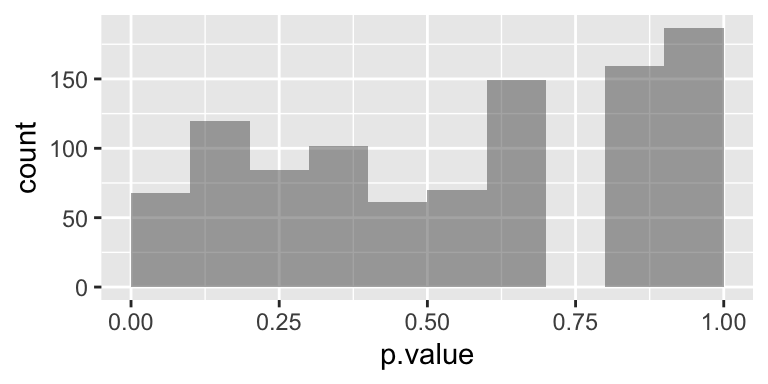
\includegraphics[width=\maxwidth]{figure/unnamed-chunk-45-1} 

}



\end{knitrout}
\begin{knitrout}
\definecolor{shadecolor}{rgb}{0.969, 0.969, 0.969}\color{fgcolor}\begin{kframe}
\begin{alltt}
\hlkwd{qqmath}\hlstd{(}\hlopt{~} \hlstd{p.value,} \hlkwc{data} \hlstd{= Chisq.null,} \hlkwc{dist} \hlstd{= qunif)}
\end{alltt}
\end{kframe}

{\centering 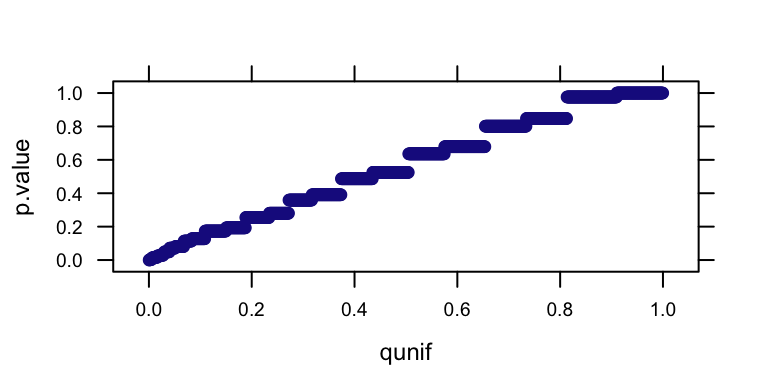
\includegraphics[width=\maxwidth]{figure/unnamed-chunk-46-1} 

}



\end{knitrout}

Perhaps more important, with the simulation approach it's straightforward to segue into more advanced and appropriate models and tests.  So, rather than the esteemed $\chi^2$ test, perhaps something a bit more modern and flexible such as logistic regression with \texttt{age} as a covariate:
\begin{knitrout}
\definecolor{shadecolor}{rgb}{0.969, 0.969, 0.969}\color{fgcolor}\begin{kframe}
\begin{alltt}
\hlstd{HELP.logistic.boot} \hlkwb{<-} \hlkwd{do}\hlstd{(}\hlnum{1000}\hlstd{)} \hlopt{*}
   \hlkwd{glm}\hlstd{(homeless}\hlopt{==}\hlstr{"homeless"} \hlopt{~} \hlstd{age} \hlopt{+} \hlstd{sex,}
     \hlkwc{data} \hlstd{=} \hlkwd{resample}\hlstd{(HELPrct),} \hlkwc{family} \hlstd{=} \hlstr{"binomial"}\hlstd{)}
\hlkwd{confint}\hlstd{(HELP.logistic.boot)}
\end{alltt}
\begin{verbatim}
##        name    lower   upper level     method estimate
## 1 Intercept -2.35771 -0.4397  0.95 percentile  -1.3846
## 2       age -0.00055  0.0479  0.95 percentile   0.0239
## 3   sexmale  0.07969  0.9428  0.95 percentile   0.4920
\end{verbatim}
\end{kframe}
\end{knitrout}

\section{Acknowledgments}

Thanks to Sarah Anoke for comments on a draft, as well as to Robin
Lock of St. Lawrence University for organizing the resampling demonstration
session at USCOTS 2011.

Project MOSAIC is supported by the US National Science Foundation (DUE-0920350).
More information about the package and this initiative can be 
found at the Project MOSAIC website: \url{www.mosaic-web.org}.

\section{Technical information}
This document was produced using R version 4.0.0 (2020-04-24) and version
1.7.0 of the \pkg{mosaic} package.

\section{References}
\begin{itemize}
\item G. W. Cobb, The introductory statistics course: a Ptolemaic curriculum?, 
   \emph{Technology Innovations in Statistics Education}, 2007, 1(1).
\item B. Efron \& R. J. Tibshirani, {\em An Introduction to the Bootstrap}, 1993, Chapman \& Hall, New York.
\item T. Hesterberg, D. S. Moore, S. Monaghan, A. Clipson \& R. Epstein.  {\em Bootstrap Methods and Permutation Tests (2nd edition)}, (2005), W.H. Freeman, New York.
\item D.T. Kaplan, {\em Statistical Modeling: A Fresh Approach}, 2nd edition, \url{http://www.mosaic-web.org/StatisticalModeling}.
\item S.C. Mednicj, D. J. Cai, J. Kanady, S. P. Drummond.  ``Comparing the benefits of caffeine, naps and placebo on verbal, motor and perceptual memory", {\em Behavioural Brain Research}, 2008, 193(1):79-86.
\item T. Speed, ``Simulation", \emph{IMS Bulletin}, 2011, 40(3):18.
\end{itemize}

\end{document}
